\chapter{System Dynamics: The Α-Ω Phase Space}
\label{ch:system-dynamics}


The SORT framework provides anatomy---a static, high-resolution snapshot of civilizational axiological code. But civilizations are not static objects. They are dynamic systems in constant motion.

\vspace{0.5em}

To diagnose health and predict trajectory requires physics.

\vspace{0.5em}

\Cref{ch:sort-framework} introduced two complementary lenses for viewing the four SORT axes. The \textbf{Philosopher's Lens} grouped them as Axiological (S-T) and Operational (R-O) planes to explain \textit{why each axis exists}. For understanding civilizational \textit{motion}, the \textbf{Engineer's Lens} proves more useful: the R-T plane (Reality + Telos) functions as the ``Axiological Engine,'' while the S-O plane (Sovereignty + Organization) forms the ``Architecture of Power.''

This chapter employs the Engineer's Lens to reveal the functional physics of dynamics.

\vspace{0.5em}

The framework predicts civilizations should cluster into distinct, recurring configurations rather than scatter randomly across the theoretical possibility space. Examining historical trajectories across diverse civilizations (\Cref{app:case-studies}) supports this prediction: one quadrant remains conspicuously, persistently empty.

What explains this clustering? What variables capture this pattern? What constraints produce it? What forces drive civilizations through this space?

\needspace{10\baselineskip}
\section{\texorpdfstring{\textbf{The Master Variables}}{The Master Variables}}\label{the-master-variables}

Two orthogonal measures compress the four-dimensional SORT complexity into analyzable dynamics.

\needspace{8\baselineskip}
\subsection{\texorpdfstring{\textbf{Ω (Omega): The Coherence Variable}}{Ω (Omega): The Coherence Variable}}\label{omega-coherence}

State Coherence\index{Omega@$\Omega$ (Coherence)} measures a polity's internal axiological alignment on a scale from 0 to 1.

\begin{definition}{State Coherence ($\Omega$)}
A quantitative measure of internal axiological unity. High $\Omega$ indicates synergistic alignment; low $\Omega$ indicates internal civil war. Calculated from axiological variance across constituent tribes: $\Omega = 1 - \sigma_A$ (power-weighted for Chimera states; see \Cref{app:scoring-rubrics}).
\end{definition}

Two engines of identical power: one mounted in aligned parts transmits force efficiently; the other, bolted to warped components, wastes energy in friction and self-destruction. This is high-Coherence versus low-Coherence.

\vspace{0.5em}

Tribes clustered together in SORT space yield low $\sigma_A$ and thus high Ω (coherent). Tribes scattered across SORT space yield high $\sigma_A$ and thus low Ω (civil war). Complete operationalization methodology in \Cref{app:scoring-rubrics}. Scored historical cases in \Cref{app:case-studies}.

\vspace{0.5em}

\textbf{The two poles:}

\begin{itemize}
\item \textbf{The Cauldron (Ω approaching 0):} Axiological civil war. The polity is a collection of warring factions sharing only a geographical container. Profoundly incoherent.

\item \textbf{The Crystal (Ω approaching 1):} Axiological monoculture. The polity is unified around a single, shared set of values. Profoundly coherent.
\end{itemize}

Coherence measures a polity's capacity for unified action---the structural integrity of the engine. But it does not tell us what the engine is actually doing.

\needspace{8\baselineskip}
\subsection{\texorpdfstring{\textbf{Α (Alpha): The Action Variable}}{Α (Alpha): The Action Variable}}\label{alpha-action}

The Action Vector\index{Alpha@$\Alpha$ (Action Vector)} measures a polity's empirically observed net output on a scale from -1.0 to +1.0.

\begin{definition}{Action Vector ($\Alpha$)}
An empirical measure of a civilization's net effect on the world. Positive $\Alpha$ indicates order creation (building, growth, conquest). Negative $\Alpha$ indicates order destruction (entropy, decay, parasitism). Assessed via POSIWID: what the system actually does, not what it claims.
\end{definition}

Imagine two perfectly built engines (high-Ω). One powers a factory, the other a wrecking ball. High energy, opposite effects.

Unlike the other variables, Α is not derived from internal axiology. It is observed empirically via POSIWID\index{POSIWID} (``The Purpose Of a System Is What It Does''): infrastructure built or destroyed, territory gained or lost, order created or annihilated, net effect on human flourishing.

\vspace{0.5em}

\textbf{The two poles:}

\begin{itemize}
\item \textbf{The Entropic Pole (Α < 0):} The polity destroys order. Its actions increase chaos, suffering, and complexity-reduction.

\item \textbf{The Syntropic Pole (Α > 0):} The polity creates order. Its actions increase complexity, energy, and Aliveness.
\end{itemize}

\vspace{0.5em}

Together, these two variables---one measuring internal unity, the other measuring external output---form a phase space that reveals the fundamental architecture of civilizational dynamics. Α relates to but differs from V (Vitality, \Cref{ch:sort-framework}): V measures internal health across three sub-indices (Fecundity, Productivity, Synergy), while Α measures external output. High-Α+ civilizations typically have high V, but the reverse can lag (consuming stored Vitality). Measurement requires judgment aggregating diverse indicators; see \Cref{app:scoring-rubrics} for rubric and \Cref{app:case-studies} for applications.

\vspace{0.5em}

\textbf{Falsification:} Independent raters scoring civilizations on Ω and Α should observe non-random clustering into four states. If scatter is random, the master variables fail.

\needspace{10\baselineskip}
\section{\texorpdfstring{\textbf{The Phase Space: Four States of Being}}{The Phase Space: Four States of Being}}\label{the-phase-space}

These two variables create a two-dimensional phase space. The framework predicts civilizations should cluster into four fundamental states. \Cref{app:case-studies} tests this prediction across diverse historical cases.

\begin{figure}[htbp]
\centering
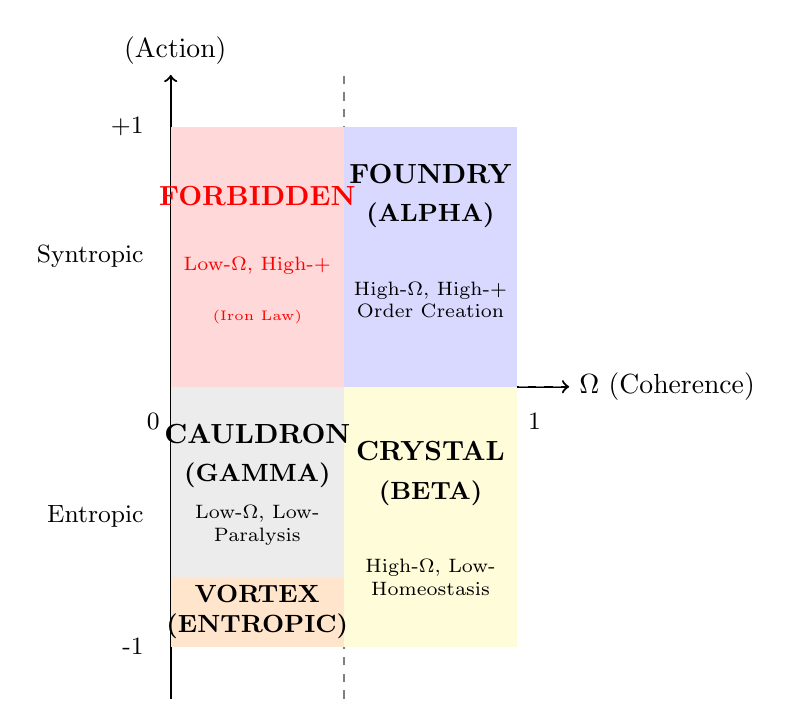
\begin{tikzpicture}[scale=2.2]
    % Axes
    \draw[->,thick] (0,0) -- (2.3,0) node[right] {$\Omega$ (Coherence)};
    \draw[->,thick] (0,-1.8) -- (0,1.8) node[above] {$\Alpha$ (Action)};

    % Axis Ticks
    \node[below] at (-0.1,-0.1) {\small 0};
    \node[below] at (2.1,-0.1) {\small 1};
    \node[left] at (-0.1,1.5) {\small +1};
    \node[left] at (-0.1,-1.5) {\small -1};

    % Axis Labels (Syntropic/Entropic)
    \node[left, align=center] at (-0.1,0.75) {\small Syntropic};
    \node[left, align=center] at (-0.1,-0.75) {\small Entropic};

    % Quadrant boundaries
    \draw[gray,thin,dashed] (1,-1.8) -- (1,1.8);
    \draw[gray,thin,dashed] (0,0) -- (2.3,0);

    % Quadrant I: ALPHA (Top-Right) - High Ω, High Α+
    \fill[blue!15] (1,0) rectangle (2,1.5);
    \node[align=center,font=\bfseries] at (1.5, 1.1) {FOUNDRY\\[2pt]\small (ALPHA)};
    \node[align=center,font=\scriptsize] at (1.5, 0.5) {High-$\Omega$, High-$\Alpha$+\\Order Creation};

    % Quadrant II: FORBIDDEN (Top-Left) - Low Ω, High Α+
    \fill[red!15] (0,0) rectangle (1,1.5);
    \node[align=center,font=\bfseries,red] at (0.5, 1.1) {FORBIDDEN};
    \node[align=center,font=\scriptsize,red] at (0.5, 0.7) {Low-$\Omega$, High-$\Alpha$+};
    \node[align=center,font=\tiny,red] at (0.5, 0.4) {(Iron Law)};

    % Quadrant IV: BETA (Bottom-Right) - High Ω, Low Α
    \fill[yellow!15] (1,-1.5) rectangle (2,0);
    \node[align=center,font=\bfseries] at (1.5, -0.5) {CRYSTAL\\[2pt]\small (BETA)};
    \node[align=center,font=\scriptsize] at (1.5, -1.1) {High-$\Omega$, Low-$\Alpha$\\Homeostasis};

    % Quadrant III: GAMMA (Bottom-Left) - Low Ω, Low Α
    \fill[gray!15] (0,-1.5) rectangle (1,0);
    \node[align=center,font=\bfseries] at (0.5, -0.4) {CAULDRON\\[2pt]\small (GAMMA)};
    \node[align=center,font=\scriptsize] at (0.5, -0.8) {Low-$\Omega$, Low-$\Alpha$\\Paralysis};

    % VORTEX as extreme sub-region of GAMMA
    \fill[orange!20] (0,-1.5) rectangle (1,-1.1);
    \node[align=center,font=\bfseries\small] at (0.5, -1.3) {VORTEX\\(ENTROPIC)};

\end{tikzpicture}
\caption{The Action-Coherence ($\Alpha$-$\Omega$) Phase Space. This maps observed civilizational outputs and reveals the empirical clustering pattern. See Figure \ref{fig:causal-phase-space} for the underlying causal structure.}
\label{fig:phase-space}
\index{phase space!Alpha-Omega@$\Alpha$-$\Omega$}
\end{figure}

\textbf{The Four Observed States:}

\begin{itemize}
\item \textbf{The Foundry (ALPHA State):} High $\Omega$, High $\Alpha$+. Coherent, high-energy, order-creating. Synergy and syntropy. \textit{Archetype:} Roman Republic (150 BC), Victorian Britain, USA (1945-1965).

\item \textbf{The Crystal (BETA State):} High $\Omega$, Low $\Alpha$ ($\approx 0$). Coherent, low-energy, homeostatic. Stable equilibrium. \textit{Archetype:} Tokugawa Japan.

\item \textbf{The Cauldron (GAMMA State):} Low $\Omega$, Low $\Alpha$ ($\approx 0$). Incoherent, low-energy, paralyzed. Internal friction and axiological civil war. \textit{Archetype:} Late Weimar Republic, Modern West.

\item \textbf{The Vortex (ENTROPIC State):} Low $\Omega$, High $\Alpha$-. Incoherent, high-energy, order-destroying. Cauldron collapsing into active self-destruction. \textit{Archetype:} Modern Haiti, Somalia (1990s).
\end{itemize}

\vspace{0.5em}

The top-left quadrant is empty. This asymmetry demands explanation.

\needspace{10\baselineskip}
\section{\texorpdfstring{\textbf{The Iron Law of Coherence}}{The Iron Law of Coherence}}\label{the-iron-law-of-coherence}

Examining historical polities reveals the Forbidden Quadrant (Low-Ω, High-Α+) remains empty. This follows from a logical argument grounded in the definitions of the variables.

Consider the conceptual constraint: What would such a civilization look like?

\vspace{0.5em}

\textbf{Low-Ω means:}
\begin{itemize}
\item Internal axiological civil war
\item Factions blocking each other
\item Massive energy wasted on internal friction
\item No sustained coordination
\end{itemize}

\textbf{High-Α+ means:}
\begin{itemize}
\item Building complex infrastructure
\item Executing long-term projects
\item Creating stable institutions
\item Coordinating large-scale action
\end{itemize}

\vspace{0.5em}

\textbf{The coordination constraint:} How do you build a cathedral when half your workers tear down what the other half builds? How do you execute a 10-year infrastructure plan when internal factions veto each other every 6 months? How do you build a starship when half your engineers sabotage the other half?

High-Α+ activities require sustained focus (impossible with internal war), institutional capacity (dissolves in low-Ω), resource pooling (factions hoard instead), high trust (antithesis of low-Ω), and long-term coordination (vetoed by opposition).

\vspace{0.5em}

This yields the Iron Law:

\begin{keyprinciple}[The Iron Law of Coherence]
\index{Iron Law of Coherence}
A polity cannot be a net creator of order in the world (High $\Alpha$+) if it is at war with itself (Low $\Omega$).

\textbf{Logical statement:} Severe internal axiological friction precludes sustained order creation.

\textbf{Mechanism:} Internal conflict dissipates the energy required for coordinated action. Low coherence precludes high output.

\textbf{Epistemic status:} Strong logical argument from the definitions of Ω and Α. The framework's empirical claim is that Ω and Α correctly model civilizational dynamics. If true, the Forbidden Quadrant should be empty in historical data.

\textbf{Falsification:} Find a sustained Low-Ω, High-Α+ civilization.
\end{keyprinciple}

\vspace{0.5em}

This is the core principle of civilizational dynamics. \textbf{Synergy is the non-negotiable precondition for Syntropy.}

Building high-Α+ states requires first establishing Ω. Without internal unity, order-creation is impossible.

\vspace{0.5em}

\textbf{Holographic Note:} This law applies to any telic system. The same physics explains personal burnout (low internal Ω attempting sustained high output), paralysis (axiological civil war consuming all available energy), and the impossibility of achieving meaningful goals while at war with yourself. \Cref{part:integrated-human} applies this principle to personal integration with the same rigor applied here to nations.

\needspace{10\baselineskip}
\section{\texorpdfstring{\textbf{The Causal Physics: From Observation to Mechanism}}{The Causal Physics: From Observation to Mechanism}}\label{the-causal-physics}

The Α-Ω diagram shows where civilizations end up. It maps observed outputs. But to understand why civilizations produce their observed outputs, we must map the causal variables: Coherence (Ω) and Telos (T).

\begin{figure}[htbp]
\centering
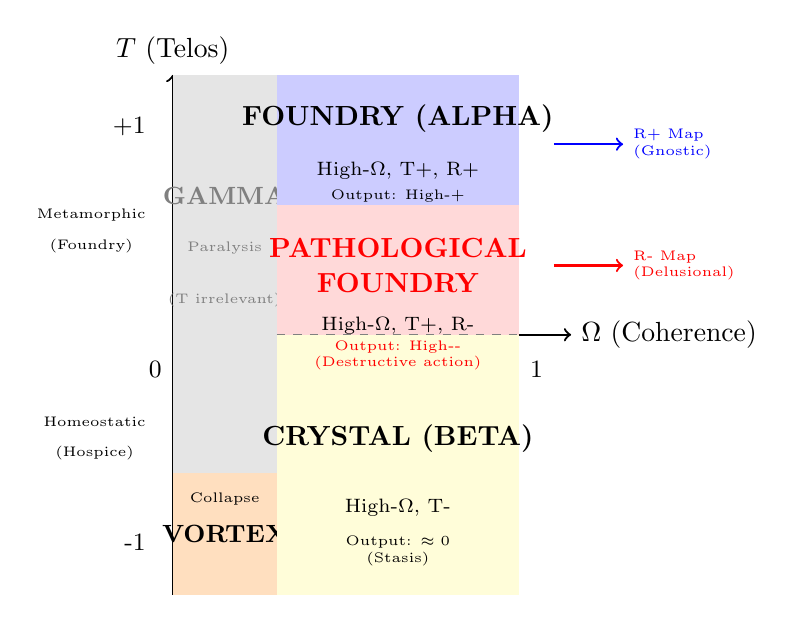
\begin{tikzpicture}[scale=2.2]
    % Axes
    \draw[->,thick] (0,0) -- (2.3,0) node[right] {$\Omega$ (Coherence)};
    \draw[->,thick] (0,-1.5) -- (0,1.5) node[above] {$T$ (Telos)};

    % Axis Ticks
    \node[below] at (-0.1,-0.1) {\small 0};
    \node[below] at (2.1,-0.1) {\small 1};
    \node[left] at (-0.1,1.2) {\small +1};
    \node[left] at (-0.1,-1.2) {\small -1};

    % Axis Labels
    \node[left, align=center] at (-0.1,0.6) {\tiny Metamorphic\\[-1pt]\tiny (Foundry)};
    \node[left, align=center] at (-0.1,-0.6) {\tiny Homeostatic\\[-1pt]\tiny (Hospice)};

    % Critical boundary line (Iron Law threshold at Ω ≈ 0.3)
    \draw[red,thick,dashed] (0.6,-1.5) -- (0.6,1.5);
    \node[red,font=\tiny,align=center] at (0.3,0) {Iron Law\\Threshold};

    % LEFT REGION: Low-Ω (all incoherent states)
    \fill[gray!20] (0,-1.5) rectangle (0.6,1.5);
    \node[align=center,font=\small\bfseries,gray] at (0.3,0.8) {GAMMA};
    \node[align=center,font=\tiny,gray] at (0.3,0.5) {Paralysis};
    \node[align=center,font=\tiny,gray] at (0.3,0.2) {(T irrelevant)};

    \fill[orange!25] (0,-1.5) rectangle (0.6,-0.8);
    \node[align=center,font=\small\bfseries] at (0.3,-1.15) {VORTEX};
    \node[align=center,font=\tiny] at (0.3,-0.95) {Collapse};

    % RIGHT REGION: High-Ω (coherent states, split by T)

    % Bottom-Right: High-Ω, T- (Hospice/Crystal)
    \fill[yellow!15] (0.6,-1.5) rectangle (2,0);
    \node[align=center,font=\bfseries] at (1.3,-0.6) {CRYSTAL (BETA)};
    \node[align=center,font=\scriptsize] at (1.3,-1.0) {High-$\Omega$, T-};
    \node[align=center,font=\tiny] at (1.3,-1.25) {Output: $\Alpha \approx 0$\\(Stasis)};

    % Top-Right: High-Ω, T+ (Foundry region - splits by R)
    \fill[blue!10] (0.6,0) rectangle (2,1.5);

    % Upper part: T+ with R+ (successful Foundry)
    \fill[blue!20] (0.6,0.75) rectangle (2,1.5);
    \node[align=center,font=\bfseries] at (1.3,1.25) {FOUNDRY (ALPHA)};
    \node[align=center,font=\scriptsize] at (1.3,0.95) {High-$\Omega$, T+, R+};
    \node[align=center,font=\tiny] at (1.3,0.80) {Output: High-$\Alpha$+};

    % Lower part: T+ with R- (pathological Foundry)
    \fill[red!15] (0.6,0) rectangle (2,0.75);
    \node[align=center,font=\bfseries,red] at (1.3,0.5) {PATHOLOGICAL};
    \node[align=center,font=\bfseries,red] at (1.3,0.3) {FOUNDRY};
    \node[align=center,font=\scriptsize] at (1.3,0.05) {High-$\Omega$, T+, R-};
    \node[align=center,font=\tiny,red] at (1.3,-0.12) {Output: High-$\Alpha$-\\(Destructive action)};

    % Dividing line at T=0
    \draw[gray,thin,dashed] (0.6,0) -- (2,0);

    % R-axis effect annotation
    \draw[->,thick,blue] (2.2,1.1) -- (2.6,1.1) node[right,font=\tiny,align=left] {R+ Map\\(Gnostic)};
    \draw[->,thick,red] (2.2,0.4) -- (2.6,0.4) node[right,font=\tiny,align=left] {R- Map\\(Delusional)};

\end{tikzpicture}
\caption{The Causal Phase Space: T-$\Omega$ Diagram. The T-axis (intent) and R-axis (map quality) determine the sign of $\Alpha$ (action output). This reveals the axiological source code generating observed states.}
\label{fig:causal-phase-space}
\index{phase space!T-Omega@$T$-$\Omega$}
\end{figure}

\needspace{8\baselineskip}
\subsection{\texorpdfstring{\textbf{Reading the Causal Map}}{Reading the Causal Map}}\label{reading-causal-map}

\textbf{The Iron Law Threshold (Vertical Red Line):} Below Ω ≈ 0.3, all states fail regardless of intent. The left side is the domain of GAMMA (paralysis) and VORTEX (collapse). This is the Iron Law of Coherence made visual.

\textbf{The High-Ω Region (Right Side):} Coherent civilizations. Their fate depends on their T-axis (intent):

\begin{itemize}
\item \textbf{T- (Homeostatic/Bottom-Right):} The BETA (Crystal) state. Goal is stasis. Output is Α ≈ 0. Example: Tokugawa Japan.

\item \textbf{T+ (Metamorphic/Top-Right):} The Foundry region. Goal is transformation. But this region bifurcates based on the R-axis:
  \begin{itemize}
  \item \textbf{R+ (Gnostic map):} Metamorphic energy channeled constructively → High-Α+ (ALPHA state). Examples: Roman Republic, Victorian Britain, Apollo Program.
  \item \textbf{R- (Delusional map):} Metamorphic energy channeled destructively → High-Α- (Pathological Foundry). Examples: Khmer Rouge, ISIS at peak coherence.
  \end{itemize}
\end{itemize}

\vspace{0.5em}

\textbf{The Key Insight:}

A civilization's position in T-Ω space (its axiological source code) determines its trajectory in Α-Ω space (its observed output). The T-axis (Telos) is the causal engine. The R-axis (Reality) is the steering wheel. Together they determine the sign and magnitude of Α.

\vspace{0.5em}

\textbf{Why T-Ω and not R-Ω?} Because Telos determines whether a civilization expends energy (magnitude), while Reality determines whether that energy is constructive or destructive (sign). T is the throttle, R is the steering wheel. This validates the Engineer's Lens from \Cref{ch:sort-framework}: the R-T plane (Axiological Engine) generates force vectors driving motion, while the S-O plane (Architecture of Power) determines institutional response.

\vspace{0.5em}

The Α-Ω diagram is the empirical map. The T-Ω diagram is the causal explanation. Both are necessary.

\needspace{10\baselineskip}
\section{\texorpdfstring{\textbf{The Force Field Model: SORT as Channels for Real Forces}}{The Force Field Model: SORT as Channels for Real Forces}}\label{the-force-field-model}

The SORT axes are not merely measurement dimensions---convenient coordinates for describing civilizations. They are channels for real forces that act upon civilizations.

A civilization's observed position in SORT space at any moment is the vector sum of multiple forces acting upon it:

\vspace{0.5em}

\textbf{Observed State = f(Biological Forces + Environmental Forces + Institutional Forces + Historical Momentum + External Pressures + Stochastic Shocks)}

\vspace{0.5em}

Observable forces---biological, environmental, institutional---act through the SORT dimensions, analogous to how physical forces act through spatial dimensions. At present, the framework provides directional predictions (sign and relative magnitude of forces). Quantitative force decomposition is an open research problem (\Cref{app:research}).

\needspace{8\baselineskip}
\subsection{\texorpdfstring{\textbf{Forces Through Each Channel}}{Forces Through Each Channel}}\label{forces-through-channels}

\textbf{S-Axis Forces:}
\begin{itemize}
\item Biological: Kin selection → Collective, neoteny → Individual
\item Environmental: Scarcity → Collective, abundance → Individual
\item Institutional: Taxation systems vs. property rights regimes
\item Cultural: Religious/tribal revivals vs. libertarian ideologies
\end{itemize}

\textbf{T-Axis Forces:}
\begin{itemize}
\item Biological: Young demographics → Metamorphosis, aging populations → Homeostasis
\item Environmental: Frontier availability → Metamorphosis, closed frontiers → Homeostasis
\item Institutional: Risk-tolerant capital markets vs. precautionary bureaucracies
\item Psychological: Collective hope and ambition vs. exhaustion and fear
\end{itemize}

\textbf{R-Axis Forces:}
\begin{itemize}
\item Epistemological: Scientific method diffusion → Gnosis, religious revivals → Mythos
\item Technological: Literacy, printing, internet → Gnosis capacity
\item Institutional: Universities and laboratories vs. temples and oral traditions
\item Crisis-driven: Empirical failures forcing Gnostic adaptation vs. meaning crises driving Mythic return
\end{itemize}

\textbf{O-Axis Forces:}
\begin{itemize}
\item Economic: Market complexity → Design necessary, small-scale production → Emergence viable
\item Technological: Coordination technology enabling Design vs. information asymmetry favoring Emergence
\item Institutional: Centralized power structures vs. distributed networks
\item Ideological: Central planning movements vs. spontaneous order philosophies
\end{itemize}

\vspace{0.5em}

A civilization's axiological position is the current equilibrium of these competing forces. A polity does not simply ``decide'' to be S+1, T+1, R+1, O+1. It is pushed and pulled by forces acting through these dimensions.

When diagnosing a civilization, we measure the vector sum. When engineering a civilization (\Cref{ch:anatomy-foundry}, \Cref{ch:sovereign-engine}), the goal is to redirect these forces. \Cref{app:case-studies} demonstrates force field analysis on historical transitions.

\vspace{0.5em}

\textbf{Falsification:} If force vector decomposition consistently fails to predict the directional trajectory (S+/-, O+/-, R+/-, T+/-) of axiological shifts, the force field model is falsified.

\needspace{8\baselineskip}
\subsection{\texorpdfstring{\textbf{Axiological Containers: Harness vs. Cage}}{Axiological Containers: Harness vs. Cage}}\label{harness-vs-cage}

This force field model yields a critical distinction in the design of institutions and cultures. There are two fundamentally different ways to create an axiological container:

\vspace{0.5em}

\textbf{The Harness:} Channels forces productively. Accepts that forces exist and cannot be eliminated, designs structures that redirect force into constructive paths.

Example: The American Founding's Constitutional Circuit-Breakers (filibuster, judicial review, federalism) channel T+ transformation energy without destroying stability (\Cref{ch:anatomy-foundry}).

\vspace{0.5em}

\textbf{The Cage:} Suppresses forces until catastrophic release. Attempts to eliminate forces rather than channel them, creating pressure that builds until the cage shatters.

Example: Soviet Union's suppression of market forces → black markets, inefficiency, collapse. Late-stage Hospice states suppressing Metamorphic energy → violent revolution (French Revolution, Cultural Revolutions).

\vspace{0.5em}

\textbf{The fundamental difference:}

The Cage sees forces as problems to be solved. The Harness sees forces as realities to be channeled.

The Cage believes it can achieve any axiological position through force of will and institutional design alone. The Harness recognizes that the forces acting on a polity (biological, environmental, historical) are more powerful than any ideological project, and thus must be respected and redirected, not denied.

\vspace{0.5em}

The art of civilizational engineering---explored in \Cref{part:blueprint}---is the art of designing axiological harnesses, not cages.

\needspace{10\baselineskip}
\section{\texorpdfstring{\textbf{Demonstration: Weimar Germany and the Mechanics of Inevitability}}{Demonstration: Weimar Germany and the Mechanics of Inevitability}}\label{weimar-demonstration}

To demonstrate the Force Field Model's predictive power, apply it to one of history's most studied transitions: the Weimar Republic (1919-1933) and its collapse into National Socialism.

The question: Can this analysis predict the observed axiological state from the vector sum of forces acting upon the civilization?

\needspace{8\baselineskip}
\subsection{\texorpdfstring{\textbf{Initial Conditions (1919): The Force Vectors}}{Initial Conditions (1919): The Force Vectors}}\label{weimar-forces}

Post-WWI Germany was subjected to an extraordinary convergence of force vectors, all acting simultaneously through the SORT channels.

\vspace{0.5em}

\textbf{1. Environmental Forces (Scarcity Shock)}
\begin{itemize}
\item Versailles Treaty: Massive reparations + territorial losses → acute resource scarcity
\item Hyperinflation (1923): Savings destroyed, middle class wiped out → existential economic threat
\item Force Vector: ↑↑ Scarcity pressure (↑T Metamorphosis needed, ↑S Collective for survival, ↑O Design for coordination)
\end{itemize}

\textbf{2. External Forces (Geopolitical Humiliation)}
\begin{itemize}
\item French occupation of Ruhr: Direct foreign military control of industrial heartland
\item International status collapse: From great power → defeated pariah
\item Force Vector: ↑↑ Collective resentment (↑S Collective identity, ↑T Metamorphosis to restore status)
\end{itemize}

\textbf{3. Historical Momentum (Cultural Inheritance)}
\begin{itemize}
\item Prussian militarism: 200+ years of high-O Design, high-S Collective traditions
\item Romantic nationalism: Deep R- Mythos of German Volk, blood-and-soil ideology
\item Force Vector: ↑ Collective (S+), ↑ Mythos (R-), ↑ Design (O+) as inherited baseline
\end{itemize}

\textbf{4. Institutional Forces (Fragile Democracy)}
\begin{itemize}
\item Weimar Constitution: New, untested democratic system with no legitimacy
\item Political fragmentation: 20+ parties, chronic instability, coalitions collapsing
\item Force Vector: ↓ Coherence (Ω chaos), ↑ pressure for O+ Design to ``fix'' disorder
\end{itemize}

\textbf{5. Biological Forces (Demographics)}
\begin{itemize}
\item WWI losses: 2+ million dead, skewed gender ratios, traumatized veterans
\item Youth bulge: Large cohort of young men with no prospects
\item Force Vector: ↑ Collective mourning (S+), ↑ Metamorphic energy (T+ from frustrated youth)
\end{itemize}

\textbf{6. Ideological Forces (Competing Memes)}
\begin{itemize}
\item Communist threat: USSR example, German communist uprisings (Spartacist, etc.)
\item Conservative backlash: Elites seeking ``order'' against leftist chaos
\item Force Vector: ↑ pressure for authoritarian O+ Design as ``solution''
\end{itemize}

\needspace{8\baselineskip}
\subsection{\texorpdfstring{\textbf{The Prediction: Vector Sum → Expected State}}{The Prediction: Vector Sum → Expected State}}\label{weimar-prediction}

Applying the force field model, the predicted directional signature is:

\vspace{0.5em}

\textbf{Predicted Archetype}: [S+, O+, R±, T+] = Authoritarian nationalist movement seeking radical transformation through designed state power.

\vspace{0.5em}

The specific values below are illustrative force rankings (not validated quantitative predictions) to demonstrate relative magnitudes:

\begin{itemize}
\item \textbf{S}: +0.7 to +0.8 (Strongly Collective - nationalist resentment + economic desperation)
\item \textbf{O}: +0.6 to +0.7 (Design-seeking - disorder creates demand for authoritarian order)
\item \textbf{R}: +0.2 to +0.4 (Mixed - industrial/engineering competence pulling toward R+ Gnosis, while Romantic nationalism and Völkisch mythology pull toward R- Mythos, yielding the observed R± signature)
\item \textbf{T}: +0.7 to +0.9 (Intense Metamorphosis - revanchism + restoration desire)
\end{itemize}

\needspace{8\baselineskip}
\subsection{\texorpdfstring{\textbf{The Observed Outcome (1933)}}{The Observed Outcome (1933)}}\label{weimar-outcome}

The Nazi movement emerged with precisely this predicted signature:

\begin{itemize}
\item \textbf{S+ (Collective)}: Volk über alles, blood-and-soil nationalism
\item \textbf{O+ (Design)}: Führerprinzip, total state planning, top-down coordination
\item \textbf{R± (Mixed)}: Industrial/military Gnosis + Aryan Mythos pseudoscience
\item \textbf{T+ (Metamorphosis)}: ``Germany will rise again,'' Lebensraum expansion, total transformation
\end{itemize}

\vspace{0.5em}

The force field model predicts that given these force vectors, an authoritarian nationalist movement with this SORT signature had high probability. The specific individual (Hitler) was a stochastic variable, but the axiological trajectory was constrained by the forces.

The Nazi movement was not an accident. It was the mechanistically probable output of the force field acting on Weimar Germany.

\needspace{8\baselineskip}
\subsection{\texorpdfstring{\textbf{What This Demonstrates}}{What This Demonstrates}}\label{weimar-implications}

\begin{enumerate}
\item \textbf{Predictive Power}: The vector sum model correctly predicts the civilizational trajectory from force decomposition.

\item \textbf{Falsifiability}: If Weimar had adopted libertarian individualism (S-) under these forces, the model would be falsified.

\item \textbf{Engineering Implications}: To prevent such outcomes, you must redirect the forces, not merely ``choose better values.''

\item \textbf{The Harness Lesson}: A civilization facing these forces needed harnesses for S+ Collective energy → productive nationalism (not expansionist revanchism), T+ Metamorphic pressure → reconstruction projects (not territorial conquest), O+ Design demand → constitutional stability (not totalitarian control).
\end{enumerate}

\vspace{0.5em}

Weimar's failure was an engineering failure: it built Cages to suppress these forces instead of Harnesses to channel them, leading to catastrophic release of energy.

This framework moves beyond moral judgment to systematic explanation. Understanding the underlying dynamics enables engineering.

\needspace{10\baselineskip}
\section{\texorpdfstring{\textbf{Falsification Conditions}}{Falsification Conditions}}\label{falsification-conditions}

The dynamic framework makes specific, testable predictions:

\begin{enumerate}
\item \textbf{Iron Law}: Find a sustained Low-Ω, High-Α+ civilization (violates coordination constraint).

\item \textbf{Clustering}: Show the observed clustering pattern doesn't exist in unbiased historical data scored by independent researchers.

\item \textbf{Trajectory prediction}: Find two civilizations with identical (Ω, Α) coordinates but radically different long-term outcomes.

\item \textbf{Force decomposition}: Demonstrate that force vector analysis yields systematically incorrect predictions of axiological trajectories.
\end{enumerate}

\vspace{0.5em}

\textbf{Epistemic Status:} This is theoretical synthesis grounded in physics, not empirical measurement. The framework's testable predictions: (1) Forbidden Quadrant remains empty across independent historical samples, (2) force vector decomposition predicts directional trajectories, (3) Ω correlates with coordinated action capacity. Initial validation across diverse historical cases (\Cref{app:case-studies}) is consistent with predictions. Whether the framework describes real constraints or proves incomplete, distributed validation will determine.

Complete methodology: \Cref{app:methodology}. Falsification protocols: \Cref{app:falsification}. Historical case studies: \Cref{app:case-studies}.

\vspace{1em}

\textbf{Part I is complete.}

You now possess both static diagnostic tools (SORT) and dynamic predictive physics (Ω-Α, Iron Law, Force Fields). You can diagnose where a civilization is (static SORT coordinates), predict where it will go (trajectory through Α-Ω phase space), and understand why certain axiological combinations are impossible (Iron Law) or inevitable (force field dynamics). You recognize that engineering civilizations requires redirecting forces through Harnesses, not suppressing them with Cages.

Part II applies this complete toolkit to the most urgent case study: the autopsy of the modern West.
